\documentclass[italian,12pt,a4paper]{article}
\usepackage[utf8]{inputenc}
\usepackage[T1]{fontenc}
\usepackage{mathtools}
\usepackage{blkarray, bigstrut} %
\usepackage{babel}
\usepackage{graphicx}
\usepackage{subfig}
\usepackage{hyperref}
\usepackage{tikz}
\usepackage{colortbl}
\usepackage{pgf-pie}
\usepackage{algorithm}
\usepackage{algpseudocode}
\usepackage{algorithmicx}
\usepackage{placeins}
\usepackage{svg}
\usepackage{tabularx}
\title{Università degli studi di Bari facoltà di scienze MM.FF.NN}
\date{} % clear date
\hypersetup{
	colorlinks=true,
	linkcolor=black,
	filecolor=magenta,      
	urlcolor=cyan,
	pdfpagemode=FullScreen,
}
\graphicspath{ {./img/} }
\RequirePackage[subfigure]{tocloft}

\cftsetindents{section}{0em}{2em}
\cftsetindents{subsection}{0em}{2em}

\renewcommand\cfttoctitlefont{\hfill\Large\bfseries}
\renewcommand\cftaftertoctitle{\hfill\mbox{}}

\algrenewcommand\algorithmicrequire{\textbf{Input:}}
\algrenewcommand\algorithmicensure{\textbf{Output:}}

\setcounter{tocdepth}{2}
\begin{document}
	\maketitle
	\thispagestyle{empty}
	\begin{center}
		\huge	\textbf{Progetto Data Mining} \\
		\Large \textbf{NASA - Nearest Earth Objects hazard detection}
	\end{center}
	
	
	
	\begin{center}
		by \\
		\Large \textbf{Vito Proscia mat. 735975}
	\end{center}

	
	\begin{figure}[hb]
		\centering
		
\includegraphics[width=5cm]{image.png}
	\end{figure}
	
	\vfill
	\begin{center}
		Anno accadenico 2022-2023
	\end{center}
	
	\newpage
	
	\tableofcontents

	\newpage

	
	\section{Introduzione}

	\subsection{Contesto}

	\href{https://www.kaggle.com/datasets/sameepvani/nasa-nearest-earth-objects/}{Near-Earth Objects} (NEO) dataset contiene una serie di informazioni, raccolte dalla NASA, che caratterizzano degli oggetti rilevati vicino alla terra, molti di questi oggetti sono a migliaia di chilometri dalla superficie terrestre, ma su scala astronomica queste distanze sono molto piccole e possono influenzare fenomeni naturali, quali per esempio cambiamenti nella marea, eventi sismici, cambiamento atmosferico, variazioni magnetiche e così via. \\
	È importante sottolineare che la maggior parte dei corpi celesti che passano vicini alla Terra sono di piccole dimensioni e passano ad una distanza sicura, solitamente non hanno un impatto significativo sui fenomeni naturali, ma quelli di dimensioni maggiori o che si avvicinano molto possono avere degli effetti. \\
	\linebreak
	La natura dei Near-Earth Objects (NEO) si può dividere in:
	\begin{itemize}
		\item \textbf{Comete}: corpo celeste relativamente piccolo, composto da gas ghiacciati frammenti di rocce e metalli.
		\item \textbf{Asteroidi}: corpi minori di un sistema planetario originati dallo stesso processo di formazione dei pianeti ma le cui fasi di accrescimento si sono interrotte più o meno presto, oppure formati attraverso la collisione tra altri corpi celesti, sono composti principalmente da silicati di nichel, ferro e magnesio.
	\end{itemize}

	
	\subsection{Definizione obiettivo principale}
	L'obiettivo principale del progetto è quello di addestrare un modello per andare a predire, in base ad alcuni parametri, quali corpi celesti rilevati attorno alla terra possono provocare danni, questo perchè è ormai ampiamente accettato dalla comunità scientifica che le collisioni di asteroidi con la Terra avvenute in passato hanno avuto un ruolo significativo nel disegnare la storia geologica e biologica del pianeta, per questo risulta interessante effettuare un task di classificazione binaria che coinvolge la feature \textit{hazardous} con classi:
	\begin{itemize}
		\item \textbf{True}: oggetto potenzialmente pericoloso.
		\item \textbf{False}: oggetto non pericoloso.
	\end{itemize}
	Inoltre si vogliono comparare le prestazioni di vari modelli addestrati con tecniche diverse per evidenziare la differenza nell'addrestamento utilizzando un dataset fortemente sbilanciato.
	In particolare si applicheranno tecniche di bilanciamento delle classi (\textit{resampling}) che agiscono sui dati e tecniche di addestramento che vanno a considerare lo sbilanciamento (\textit{cost-sensitive learning}) che riguardano più la controparte algoritmica. \\
	Avremo, quindi da sperimentare algoritmi di learning Cost-insensitive e Cost-sensitive (meta) sul dataset originale, il dataset sul quale è applicato il resampling con \textit{SMOTEENN} e quello sul quale è applicato \textit{ADASYN}.
	
	\subsection{Metodologia}
	
	Per raggiungere lo scopo si è utilizzato il CRISP-DM (CRoss Industry Standard Process for Data Mining), una metodologia per attuare il KDD (Knowledge Discovery from Data).
	
	\begin{figure}[h]
		\centering
		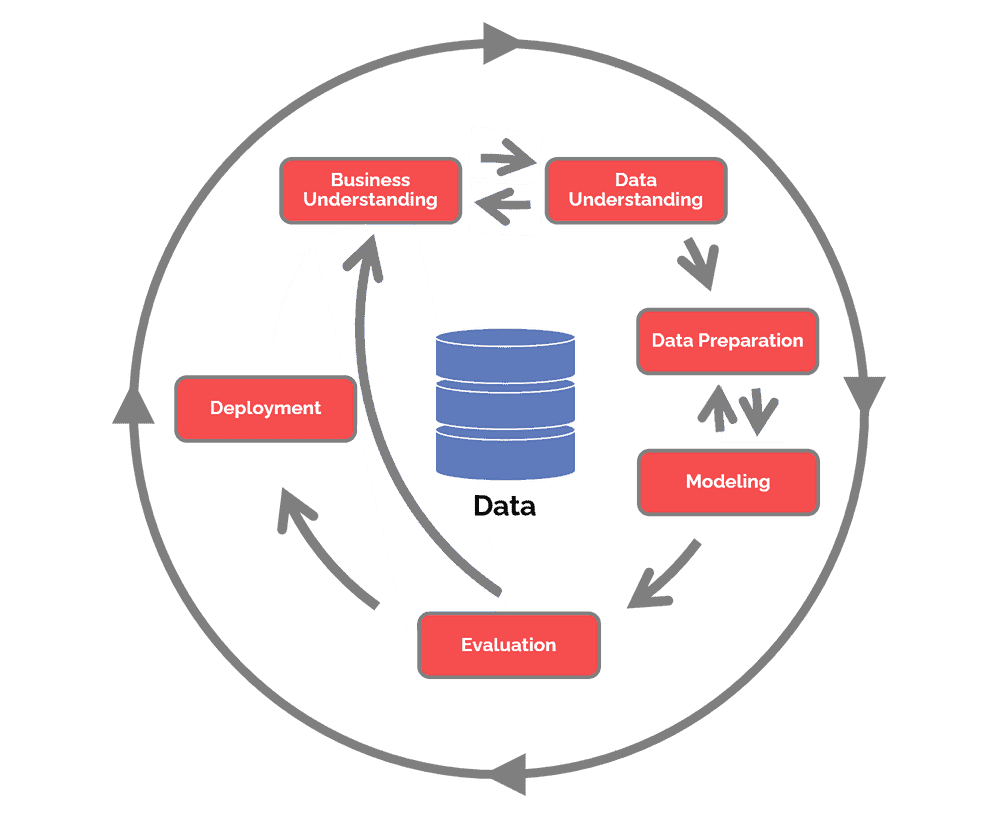
\includegraphics[scale=0.3]{CRISP-DM}
	\end{figure}

	In particolare il CRISP-DM si compone di sei fasi:
	
	\begin{enumerate}
		\item \textbf{Buisness understanding}, dove si studia e si comprende il dominio applicativo e gli obiettivi da raggiungere, andando a produrre un project plan.
		\item \textbf{Data understanding}, fase nella quale si identificano metodi per l'acquisizione dei dati, problemi legati a quest'ultimi, come la qualità, gli errori, etc.., quì avviene la fase di esplorazione preliminare del dataset.
		\item \textbf{Data preparation}, preparazione del dataset(s) andando a determinare il sottoinsieme dei dati che più rappresenta il dataset in funzione degli obiettivi, pulendo il dataset da errori, valori mancanti, \textit{outliers} ed attributi non funzionali allo scopo (feature selection), attuare tecniche per andare a ribilanciare i dati e così via.
		\item \textbf{Modeling}, fase in cui si selezionano le tecniche di modeling andando a scegliere gli algoritmi da provare ed eseguendoli con i dovuti parametri, per poi andare a valutarli con le opportune metriche.
		\item \textbf{Evaluation}, fase di confronto fra il data scientist ed il buisness owner per andare a valutare i risultati ottenuti in relazione agli obiettivi di buisness.
		\item \textbf{Deployment}, fase finale di messa in produzione del modello selezionato.
	\end{enumerate}

	Il CRISP-DM è un metodo \textit{agile}, quindi le fasi scandite precedentemente non sono da considerare rigide, da applicare una dopo l'altra, ma si può, in caso di necessità, ritornare indietro da qualsiasi fase, rendendo, quindi, il processo molto flessibile.
	
	\subsection{Tool utilizzati}
	Per la sperimentazione sono stati usati diversi stumenti, quali:
	
		\begin{itemize}
			\item \href{https://colab.research.google.com/}{Google Colab}, strumento  presente nella suite Google che consente di scrivere python notebook direttamente dal proprio browser, utilizzando risorse messe a disposizione da remoto. 
			\item \href{https://www.cs.waikato.ac.nz/~ml/weka/}{Weka}, software contenente una collezione di algoritmi per data Mining e apprendimento Automatico, scritto in Java e sviluppato presso University of Waikato New Zealand.
			\item \href{https://code.visualstudio.com/}{Visual Studio Code}, editor di codice.
		\end{itemize}


	\section{Analisi del dataset}
	
	\subsection{Descrizione features}
	Il dataset inizialmente si compone di 90836 osservazioni per dieci features che vanno a descrivere una serie di caratteristiche dei corpi celesti registrati, in particolare abbiamo:
	
	\begin{enumerate}
		\item \textit{id} [numeric]: identificatore univoco per ogni oggetto.
		\item \textit{name} [string]: nominativo dato dalla NASA.
		\item \textit{est\_diameter\_min} [numeric]: diametro minimo stimato (Km).
		\item \textit{est\_diameter\_max} [numeric]: diametro massimo stimato (Km).
		\item \textit{relative\_velocity} [numeric]: velocità relativa rispetto alla terra (Km/h).
		\item \textit{miss\_distance }[numeric]: distanza minima tra il NEO e la Terra durante il suo passaggio più ravvicinato (Km/h).
		\item \textit{orbiting\_body} [string]: corpo rispetto al quale l’oggetto sta orbitando.
		\item \textit{sentry\_object} [boolean]: copro incluso o meno in sentry (sistema di monitoraggio automatico delle collisioni).
		\item \textit{absolute\_magnitude} [numeric]: descrizione della luminosità dell’oggetto (energia radiata dal corpo al secondo).
		\item \textit{hazardous} [boolean]: indica se il corpo è pericoloso o meno.
	\end{enumerate}
	
	\subsection{Preparazione dati}
	
	\subsubsection{Analisi delle input features}
	Andando a considerare direttamente il dataset come ci vine fornito ci sono una serie di problematiche legate ad alcune features, alcune di queste sono inutili per lo scopo di addestramento, quali: 
	
	\begin{itemize}
		\item \textit{id} (nessuna correlazione con la feature su cui fare predizione).
		\item \textit{name} (nessuna correlazione con la feature su cui fare predizione).
		\item \textit{orbiting\_body} (ha un unico valore).
		\item \textit{sentry\_object} (ha un unico valore).
	\end{itemize}
	
	
	\subsubsection{Analisi della target feature}
	Lo scalido piò arduo da affrontare riguarda sicuramente la natura delle osservazioni inerenti alla target feature \textit{hazardous}, che presenta una distrubuzione di valori fortemente sbilanciata ($90.3\%$ per False e $9.7\%$ per True) per via della natura della osservazioni e del dominio a cui fanno riferimento.
	
	\begin{center}
		\begin{figure}[!ht]
			\centering
			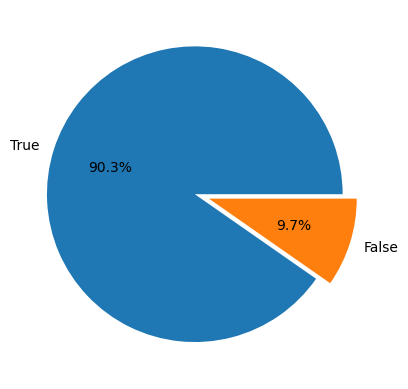
\includegraphics[scale=0.73]{imbcalss}
		\end{figure}
	\end{center}

	\section{Resampling per lo sbilanciamento delle classi}
	Il resampling è un tecnica (data driven) usata per bilanciare le osservazioni di ogni classe andando a generarne di nuove o eliminandole per risolvere il problema dello sblianciamento.
	
	\subsection{Oversampling vs Undersampling}

	L’oversampling e l’undersampling sono due metodi per andare a risolvere lo sbilanciamento delle classi target, in particolare l’undersampling prevede il ridimensionamento di una classe prelevando da una popolazione un suo sottoinsieme, questo si applicherebbe alla classe più numerosa, mentre l’oversampling sposta il focus sulla classe con meno occorrenze andando a creare “sinteticamente” delle nuove osservazioni a partire da quelle già a disposizione.
	
	\subsection{Approccio ibrido}
	Nel nostro caso, come già accennato, le classi della target feature \textit{hazardous} (true/false) sono molto sbilanciate (causa del fatto che per fortuna sono pochi i corpi celesti che si rivelano potenzialmente pericolosi), se da una parte i \textit{false} superano gli 80k, dall'altra i \textit{true} arrivano a malapena a 8k, quindi se applicassimo una tecnica di undersampling si avrebbe un’enorme perdita di informazioni, mentre se usassimo l’oversampling, per bilanciare i dati avremo moltissimi dati sintetici, per questo sarebbe meglio usare una tecnica ibrida.
	\linebreak
	\subsubsection{SMOTE-ENN}
	L’algoritmo SMOTE-ENN [Batista et al 2004] combina l’abilità di SMOTE (Synthetic Minority Oversampling)  di generare istanze sintetiche per la classe minoritaria, con quella di ENN (Edited Nearest Neighbor) [Wilson 1972] di eliminare da entrambe le classi alcune osservazioni. \\
	\linebreak
	L'algoritmo, come dice il nome, è basato su SMOTE, tecnica usata per la creazione di istanze sintetiche della classe minoritaria, andando ad aggiungere nuove istanze con valori mediati tra i $k$ vicini di una osservazione della classe, proprio per questo, teoricamente, nella nostra situazione non dovrebbe performare troppo bene, avendo le istanze della classe minoritaria molto vicine a quella della classe maggioritaria, creando così istanze sintetiche con valori mediati tra classi diverse.
	
	\begin{algorithm}
		\caption{SMOTE-ENN}
		\begin{algorithmic}
			\Require $Tr$ : Training set, \\ $p$: number of nearest neighbors in SMOTE, \\ $k$: number of nearest neighbors in ENN
			\Ensure $New\_Tr$ : Training set after using SMOTE-ENN \\
			\textbf{1.} Divide $Tr$ into positive and neative subsets: \\ $Tr \leftarrow Pos \cup Neg;$  \\
			\textbf{2}. Oversampling the minority class using SMOTE to balance calss distribution: \\
			$New\_Pos \leftarrow SMOTE(Pos, p);$ \\
			$|New\_Pos| = |Neg|;$ \\
			\textbf{3.} $New\_Tr \leftarrow New\_Pos \cup Neg;$ \\
			\textbf{4.} Remove noisy examples using ENN: \\
			$New\_Tr \leftarrow ENN(New\_Tr);$
		\end{algorithmic}
	\end{algorithm}

	\begin{figure}[!ht]
		\centering
		\subfloat[Prima di SMOTE-ENN]{%
			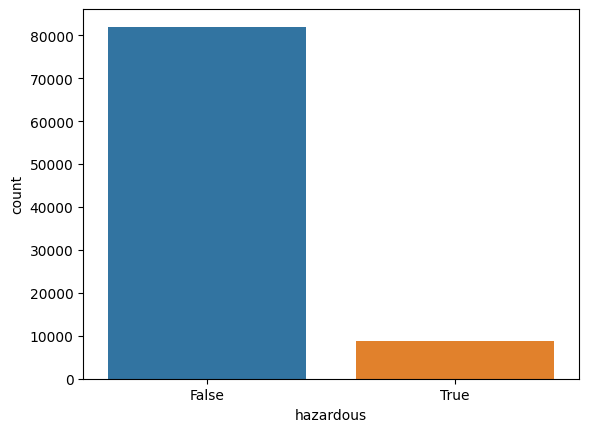
\includegraphics[scale=0.5]{imb_graph.png}%
		}%
		\subfloat[Dopo SMOTE-ENN]{%
			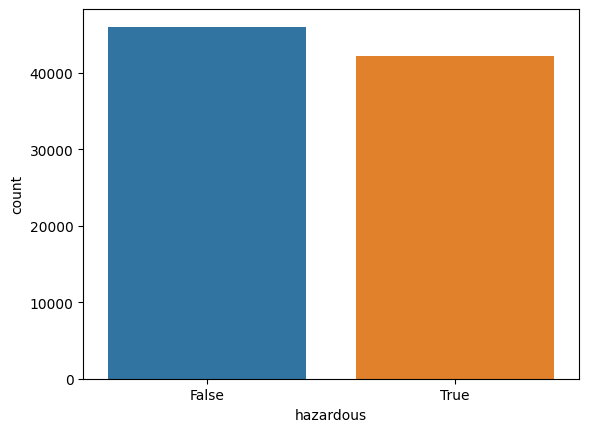
\includegraphics[scale=0.5]{smoteenn_graph.png}%
		}%
	\end{figure}
	\subsubsection{ADASYN}
	L'algoritmo ADASYN (Adaptive Synthetic) si basa sull'idea di generare sinteticamente dei nuovi dati per la classe minoritaria considerando la distribuzione delle osservazioni della sudetta classe. Vengono generati più dati a partire dalle osservazioni, della classe minoritaria, che sono più difficili da imparare. \\
	La chiave di ADASYN è l'uso della distribuzione dei pesi $\hat{r_i}$ come criterio per decidere quante osservazioni sintetiche creare per ogni esempio della classe minoritaria.
	
		\begin{algorithm}
		\caption{ADASYN}
		\begin{algorithmic}
			\Require $Tr$ : Training set, \\ $m\_s$: number of samples of minority class, \\ $m\_l$: number of samples of majority class.
			\Ensure $Tr\_res$ : Training set resampled \\
			\textbf{1.} Calculate the degree of class imbalance: $$d = \frac{m_s}{m_l} \in (0, 1]$$  \\
			\textbf{2}. \textbf{If} {$d < d_{th}$} ($d_{th}$ preset threshold) \\
						\quad\textbf{a)} Calculate the number of synthetic data examples that
						need to be generated for the minority class: $$G = (m_l - m_s)\beta$$
						\quad Where $\beta \in [0, 1]$ balance level after generation of the synthetic data. \\
						\quad \textbf{b)} \textbf{For each} example $x_i \in minorityClass$ find $k$ nearest neighbors and calculate: $$r_i = \frac{\Delta_i}{k} = \frac{\# majotiry\_class\_neighbors}{k}, i = 1, \dots m_s$$
						\quad \textbf{c)} Normalize $r_i$ according to: $$\hat{r_i} = \frac{r_i}{\sum_{j = 1}^{m_s} r_j}$$
						\quad \textbf{d)} Calculate the number of synthetic data examples for each $x_i$: $$g_i = \hat{r_i} G$$
						\quad \textbf{e)} \textbf{For} $1$ \textbf{to} $g_i$ \\
						\quad \quad \textbf{i)} Randomly choose one minority data example, $x_{zi}$,
						from the $k$ nearest neighbors for data $x_i$ \\
						\quad \quad \textbf{ii)} Generate the synthetic data example: $$s_i = x_i + (x_{zi} - x_i)\lambda$$
						Where $(x_{zi} - x_i)$ is the difference vector and $\lambda \in [0,1]$ is a random number. \\

		\end{algorithmic}
	\end{algorithm}
	\begin{figure}[!ht]
	\centering
	\subfloat[Prima di ADASYN]{%
		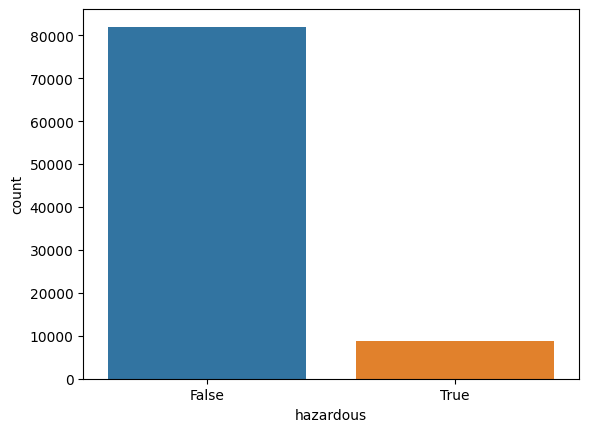
\includegraphics[scale=0.5]{imb_graph.png}%
	}%
	\subfloat[Dopo ADASYN]{%
		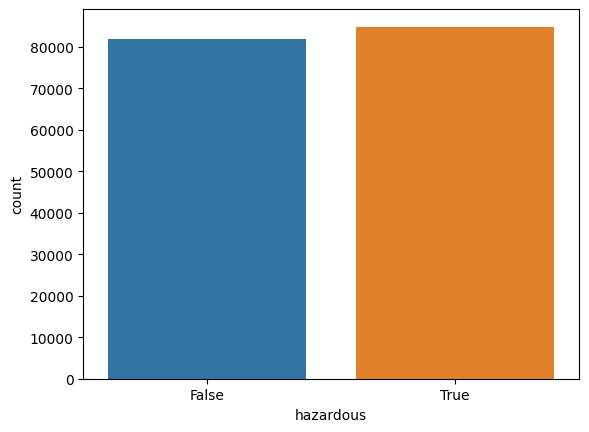
\includegraphics[scale=0.5]{adasyn_graph.png}%
	}%
\end{figure}
	
	\section{Cost-Sensitive learning per lo sbilanciamento delle classi}
	Il \textit{cost-sensitive learning} è un task di data mining che tiene in considerazione il costo di una classificazione sbagliata (\textit{misclassification cost}), andando a considerare una classificazione binaria, ad ogni tipo di predizione viene asseganto un costo, formando una \textit{cost matrix}: \\
	\begin{center}
		\begin{tabularx}{0.8\textwidth} { 
				| >{\centering\arraybackslash}X 
				| >{\centering\arraybackslash}X 
				| >{\centering\arraybackslash}X | }
			\hline
			 & Actual negative & Actual positive \\
			\hline
			Predict negative & $C(0, 0)$ TN & $C(0, 1)$ FN \\
			\hline
			Predict positive  & $C(1, 0)$ FP & $C(1, 1)$ TN \\
			\hline
		\end{tabularx}
	\end{center}

	Dove $C(i, j)$ rappresenta il costo della classificazione dove $i$ è la predizione, mentre $j$ è la classe corretta. \\
	Il cost-sensitive learning è utile in caso di sbilanciamento delle classi perchè da più peso agli errori di classificazione, in particolare nella classificazione dei FN (False Negative) cioè esempi classificati come \textit{false} ma che in realtà sono \textit{true}.
	
	\subsection{Threshold factor}
	Il \textit{threshold factor} è un valore soglia che consente la classificazione di una osservazione $x$ in \textit{true} (assumendo che la classe minoritaria sia quella con valori \textit{true}). \\
	In particolare: $$p* = \frac{FP}{FP + FN} = \frac{C(1, 0)}{C(1, 0) + C(0, 1)}$$
	Se $P(true, x) \ge p*$ allora $x$ viene classificato come \textit{true}.
	
	\subsection{Meta Learning}
	Il \textit{meta learning} è un tipo di \textit{cost-sensitive learning} che converte un algoritmo \textit{cost-insensitive} in uno \textit{cost-sensitive} in due modi diversi:
	
	\begin{itemize}
		\item \textbf{Threshold}, usa la soglia $p*$ per la classificazione
		\item \textbf{Sampling}, modifica della distribuzione dei dati per poi andare ad applicare un algoritmo di learning
	\end{itemize}
	
	\section{Machine Learning}
	Tenendo conto di tutte le considerazioni fatte, la parte inerente all'addestramento ed alla successiva valutazione si concentrerà in particolare sulle differenze tra l'addestramento su tre instanze del dataset, in particolare con il dataset originale, il dataset su cui è eseguito l'algorimto SMOTE-ENN ed il dataset su cui è eseguito ADASYN, andando a differenziare tra cost-insensitive learning e cost-sensitive learning.
	
	
		\begin{figure}[!h]
			\centering
			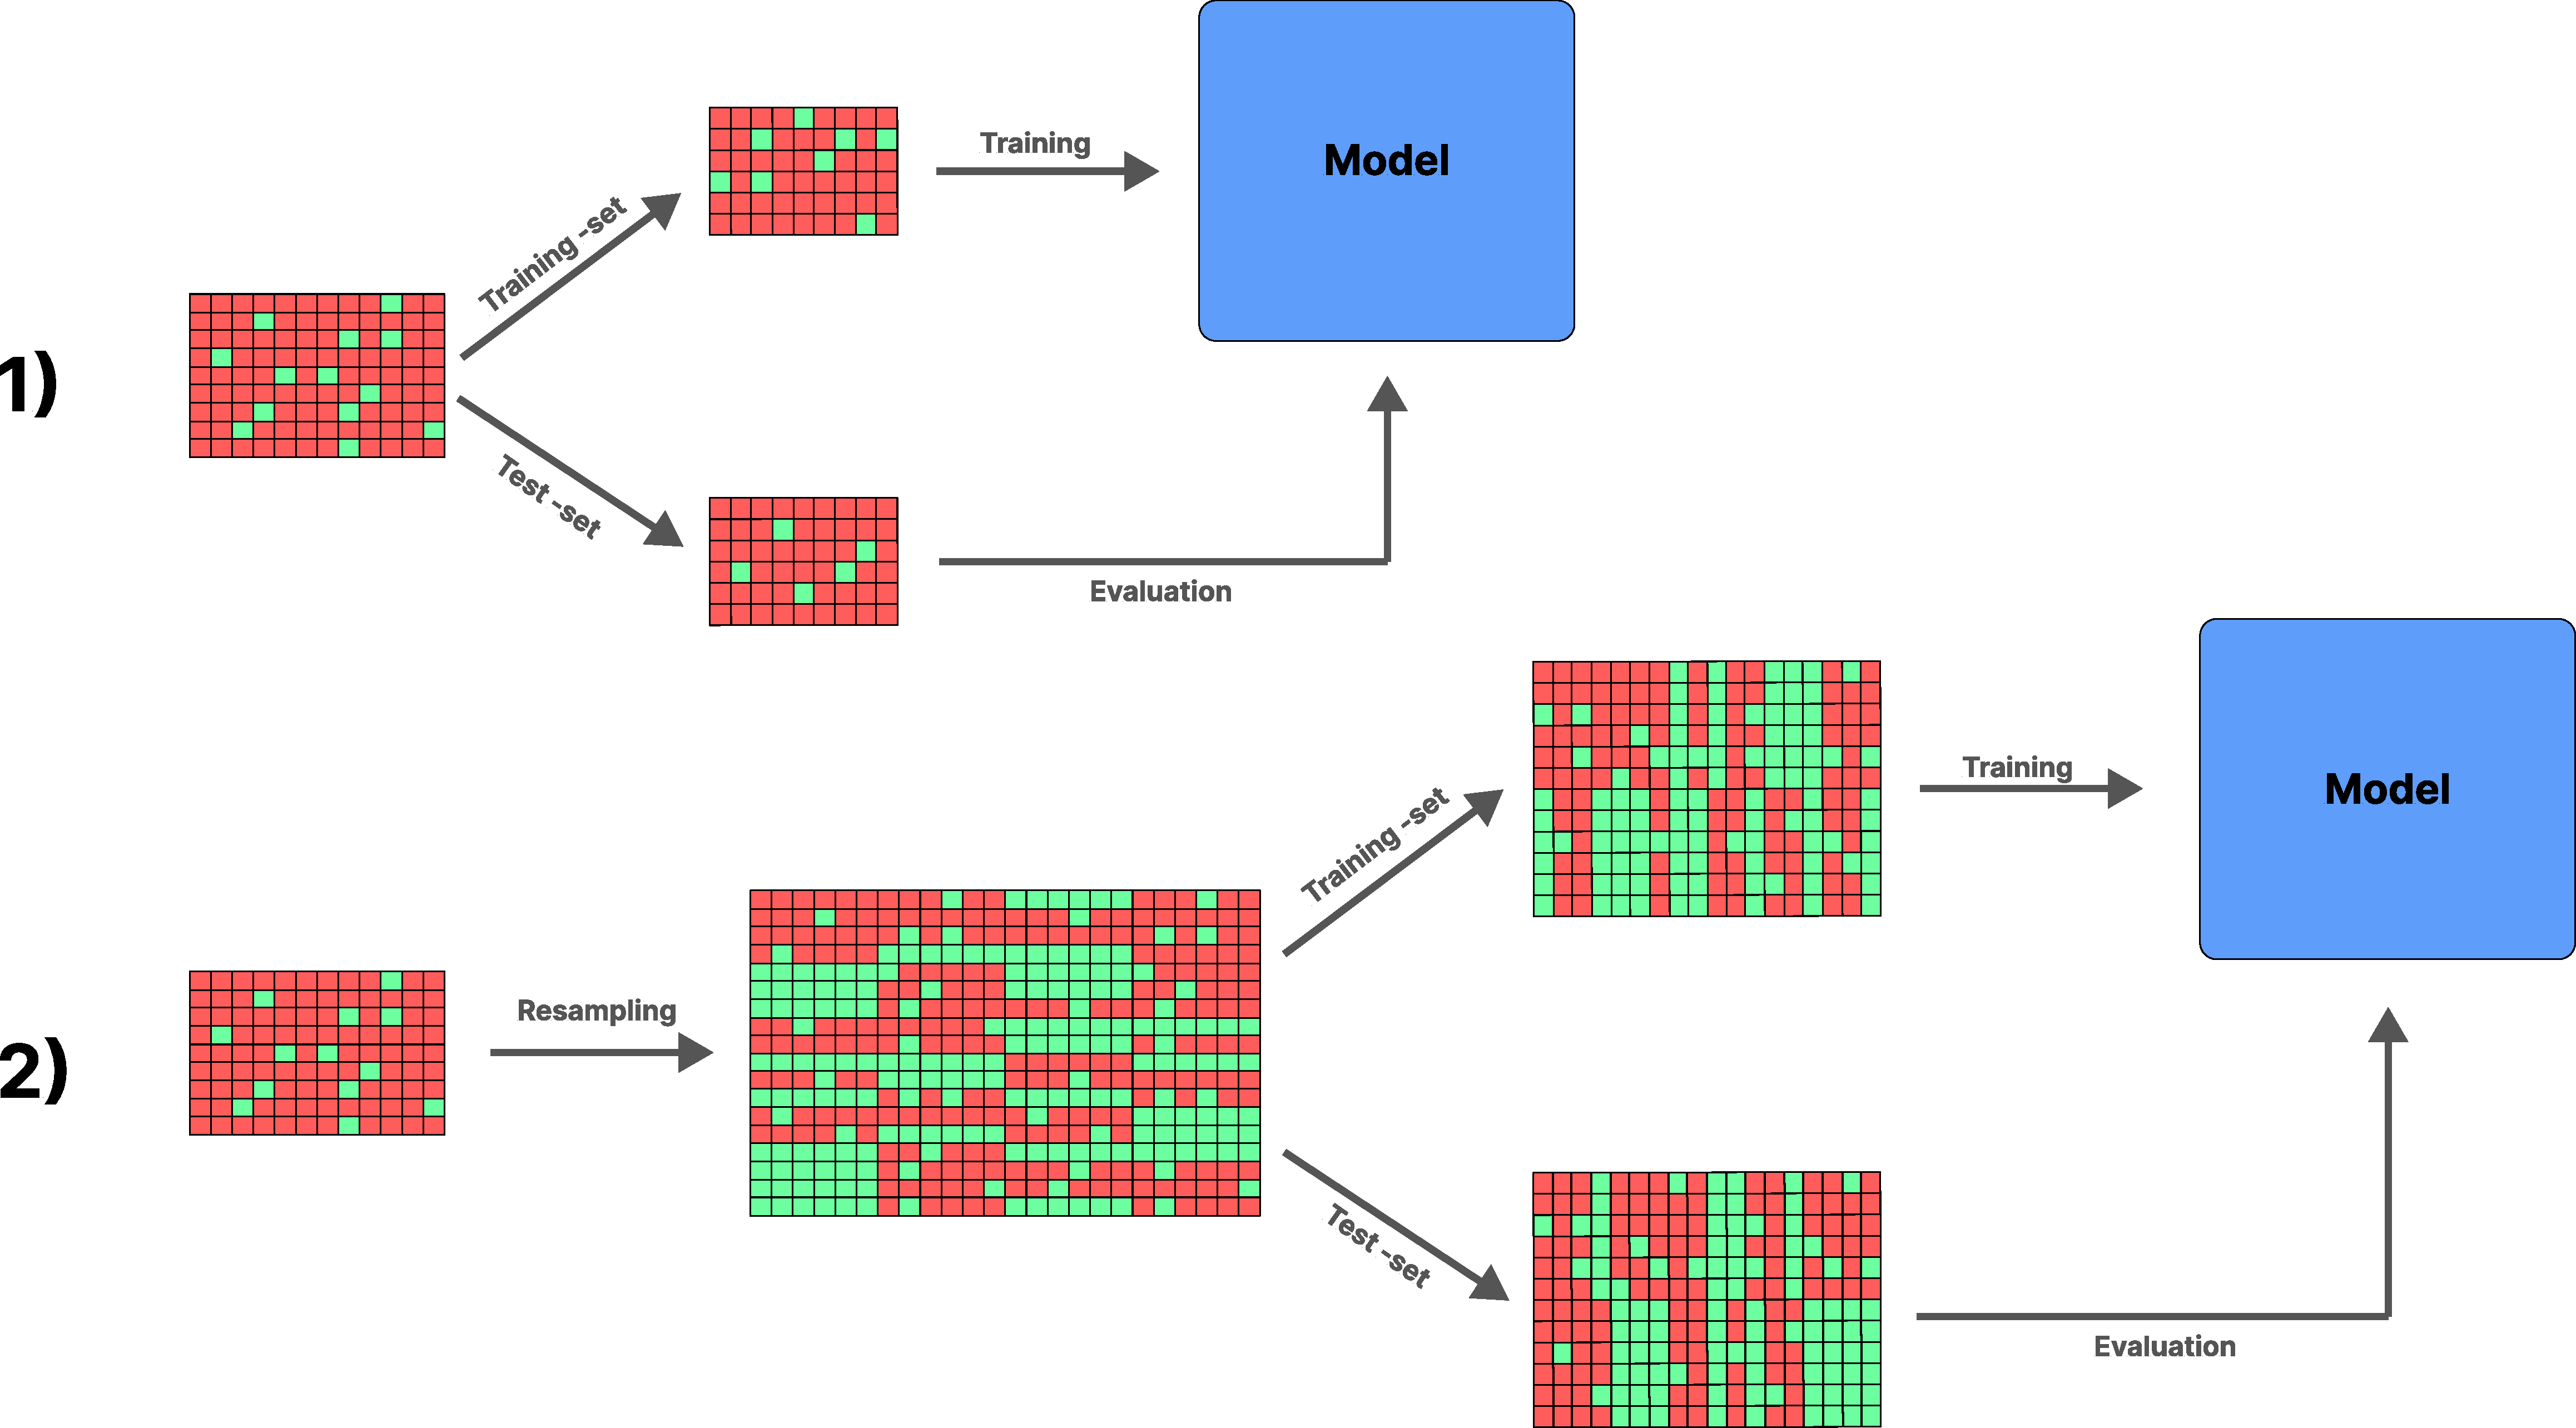
\includegraphics[width=15cm]{metodology_graph}
		\end{figure}
		
	\subsection{Modelli di learning}
	L'addestramento avverrà principalmente con due modelli di learning:
	
	\begin{itemize}
		\item Albero di calssificazione, in particolare il C4.5
		\item Naive Bayes
	\end{itemize}
	   
	\subsubsection{Classification Tree C4.5}
	Modello di classificazione che prende in input una collezione di esempi di training $S$ e l'iniseme delle classi $C = \{c_1, c_2, \dots, c_k\}$, ad ogni nodo dell'albero, C4.5 sceglie l'attributo dei dati che più efficacemente suddivide $S$ insieme di campioni in sottoinsiemi in base alle classi. Il criterio di suddivisione è \textit{l'information gain} (differenza di entropia). L'attributo con il più alto guadagno di informazioni normalizzate viene scelto per prendere la decisione. \\
	\textit{l'information gain} per l'attributo di test $t$ sarà:
	
	$$IG(S, t) = E(S) - \sum_i \frac{|S_i|}{|S|}E(S_i)$$ dove $$E(S) = -\sum_{i = 1, \dots, k} Count(c_i, S)\cdot\log(Count(c_i, S))$$
	
	Nel nostro caso abbiamo allenato il modello con sei configurazioni:
	
	\begin{itemize}
		\item \texttt{DecisionTreeClassifier().fit(X\_train, y\_train)}, classificatore cost-insensitive addesstrato su il dataset originale, il dataset ribilanciato con SMOTEENN e il dataset ribilanciato con ADASYN.
		\item \texttt{DecisionTreeClassifier(class\_weight="balanced").fit(X\_train, y\_train)}, classificatore cost-sensitive addestrato su il dataset originale, il dataset ribilanciato con SMOTEENN e il dataset ribilanciato con ADASYN.
		
	\end{itemize}
	
	N.B. L'attributo \texttt{class\_weight} è stato impostato a \texttt{"balanced"} per andare a regolare automaticamente i pesi in modo inversamente proporzionale alle classi: $$w_{true} = \frac{N_s}{2\cdot N_{true}} \quad w_{false} = \frac{N_s}{2\cdot N_{false}} $$ dove $N_s$ è la cardinalità del dataset, $2$ rappresenta il numero di classi, $N_{true}$ e $N_{false}$ sono rispettivamente il numero di occorrenze con classe \textit{true} e con classe \textit{false}.
	
	\subsubsection{Naive Bayes}
	
	Il naive bayes è uno dei modelli del framework bayesiano, si basa sul teorema di Bayes:
	$$P(h|D) = \frac{P(D|h)\cdot P(h)}{P(D)}$$
	Più nello specifico il naive Bayes, considerando ogni instanza del dataset come una tupla di valori $<a_1, a_2, \dots, a_n>$ e l'attributo target che prende i valori da un insieme $V$, va a stimare $P(v_j)$, cioè la probabilità a priori che l'attributo target abbia valore $v_j$, con la frequenza relativa del valore $v_j$ nel dataset $$P(v_j) = \frac{\#istanze\_con\_val\_v_j}{\#istanze\_tot}$$ similmente andrà a stimare la probabilità condizionata $P(a_i|v_j)$ contando quante occorrenze classificate con $v_j$ hanno il valore $a_i$. \\
	Andando ad assumere l'indipendenza condizionale dei valori degli attributi, avremo:
	$$V_{NB} = \max_{v_j \in V}(P(v_j)\prod_{i = 1}^{n} P(a_i|v_j))$$
	Quindi all'istanza $x$ verrà assegnata la classe $v_j$ che ha massimizzato il valore sopra citato. \\
	Nel nostro caso abbiamo allenato il modello con i tre dataset, dataset originale, il dataset ribilanciato con SMOTEENN e il dataset ribilanciato con ADASYN.
	
	\section{Valutazione dei modelli}
	Per andare a valutare i modelli prodotti dopo l'addestramento si è usata la k-Fold-Cross-Validation, che esegue la ripartizione del dataset $D$ in k sottoinsiemi (folds), $D_1, D_2, \dots, D_k$ prevede $k$ iterazioni ed all'$i$-esima iterazione il sottoinsieme $D_i$ sarà usato come dataset di test, metre l'unione degli altri sarà usata per allenare il modello.
	
	\subsection{Metriche scelte}
	Ai fini della valutazione si hanno a disposizione moltissime metriche adatte per moltissime situazioni, le più comuni sono
	
	$$Precision = \frac{TP}{TP+FP} \quad Recall = \frac{TP}{TP+FN}$$
	
	ma nel nostro caso, avendo un dataset fortemente sbilanciato, non bastano, per questo ci si concentrerà principalmente su:
	
	\begin{itemize}
		\item $f\beta-score$,  combinazione delle metriche classiche di $precision$ e $recall$ bilanciate da un parametro $\beta$ nella media armonica.
		$$f\beta-score = \frac{(1+ \beta^2) \cdot Precision \cdot Recall}{\beta^2 \cdot Precision + Recall}$$
		\item $ROC Area$, area sotto la curva che rappresenta la relazione tra il tasso di veri positivi (True Positive Rate, TPR) e il tasso di falsi positivi (False Positive Rate, FPR) al variare della soglia di classificazione.
			$$TPR = \frac{TP}{TP+FN} \quad FPR = \frac{FP}{FP+TN}$$
		la $ROC Area$ è particolarmente utile per valutare modelli addestrati su dataset sbilanciati perché non è influenzata dalla distribuzione delle classi nel dataset, infatti misura la capacità del modello di classificare correttamente gli esempi positivi rispetto a quelli negativi, indipendentemente dal numero di esempi in ciascuna classe.
	\end{itemize}

	\section{Risultati}
	
	In questa sezione verranno riportati tutte le metriche discusse per ogni modello, separando per tipo di dataset e per tipo di algoritmo.\\
	Matrice di costo usata, con pesi calcolati dalla formula precedente:
	
		\begin{center}
			 \begin{blockarray}{*{2}{c} l}
				\begin{block}{*{2}{>{$\footnotesize}c<{$}} l}
				Actual\_negative & Actual\_positive & \\
				\end{block}
				\begin{block}{[*{2}{c}]>{$\footnotesize}l<{$}}
				0 & 0.55 & Predict\_negative \\
				5.13 & 0& Predict\_negative \\
				\end{block}
			\end{blockarray}		
		\end{center}
	

	
	\subsection{Classification Tree C4.5}
	
	\subsubsection{Cost-insensitive learning}

	
	\begin{center}
	
	   \begin{table}[h]
		\footnotesize
		\begin{tabular}{|p{2cm}|c|}
			\hline
			\multicolumn{2}{|c|}{Dataset originale}\\ \hline
				Accuracy & 0.889 \\ \hline
				Precision & 0.441 \\ \hline
				Recall & 0.448 \\ \hline
				F-measure macro & 0.692 \\ \hline
				ROC Area & 0.693 \\ \hline
		\end{tabular}
		\hfill
		\begin{tabular}{|p{2cm}|c|}
			\hline
			\multicolumn{2}{|c|}{SMOTEENN}\\ \hline
				Accuracy & 0.927 \\ \hline
				Precision & 0.922 \\ \hline
				Recall & 0.925 \\ \hline
				F-measure macro & 0.927 \\ \hline
				ROC Area & 0.927 \\ \hline  
		\end{tabular}
		\hfill
		\begin{tabular}{|p{2cm}|r|} \hline
			\multicolumn{2}{|c|}{ADASYN}\\ \hline
				Accuracy & 0.938 \\ \hline
				Precision & 0.937 \\ \hline
				Recall & 0.941 \\ \hline
				F-measure macro & 0.938 \\ \hline
				ROC Area & 0.938 \\ \hline  
		\end{tabular}
	\end{table}
	
		\begin{figure}[h]
			\centering
			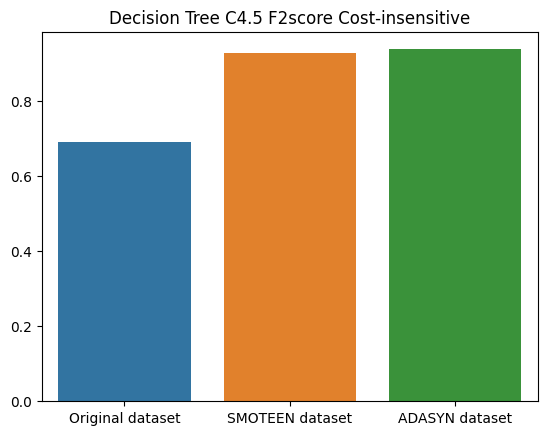
\includegraphics[scale=0.73]{DecTree}
		\end{figure}
	
	
	\end{center}
	
	Andando a valutere i risultati ottenuti possiamo notare che in tutti e tre i casi i valori dell'accuracy sono molto alti, ma questo non basta, perchè tiene conto della distribuzione delle classi, mentre le metriche di principale interesse, nel nostro caso, la $f\beta-score$ e $ROC Area$ non dipendendo dalla distribuzione delle classi sono molto più significative, infatti nel caso del dataset originale sono appena sufficienti, sui 0.69, mentre con i dataset ribilanciati sono molto più alte, quindi possimao riscontrare più o meno lo stesso miglioramento andando a ribilanciare le classi con i due algoritmi. \\
	\linebreak
	\linebreak
	
	\subsubsection{Cost-sensitive learning}
	
		\begin{center}
		
		\begin{table}[h]
			\footnotesize
			\begin{tabular}{|p{2cm}|c|}
				\hline
				\multicolumn{2}{|c|}{Dataset originale}\\ \hline
				Accuracy & 0.891 \\ \hline
				Precision & 0.446 \\ \hline
				Recall & 0.428 \\ \hline
				F-measure macro & 0.686 \\ \hline
				ROC Area & 0.685 \\ \hline  
			\end{tabular}
			\hfill
			\begin{tabular}{|p{2cm}|c|}
				\hline
				\multicolumn{2}{|c|}{SMOTEENN}\\ \hline
				Accuracy & 0.928 \\ \hline
				Precision & 0.923 \\ \hline
				Recall & 0.928 \\ \hline
				F-measure macro & 0.928 \\ \hline
				ROC Area & 0.928 \\ \hline  
			\end{tabular}
			\hfill
			\begin{tabular}{|p{2cm}|r|} \hline
				\multicolumn{2}{|c|}{ADASYN}\\ \hline
				Accuracy & 0.937 \\ \hline
				Precision & 0.937 \\ \hline
				Recall & 0.940 \\ \hline
				F-measure macro & 0.937 \\ \hline
				ROC Area & 0.937 \\ \hline  
			\end{tabular}
		\end{table}
		\begin{figure}[h]
			\centering
			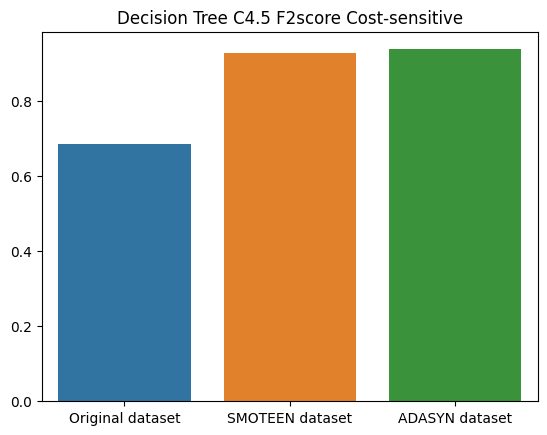
\includegraphics[scale=0.73]{DecTreeCostSens}
		\end{figure}
	\end{center}
	
	Anche per il Cost-sensitive learning con la matrice di costo definita precedentemente i valori non si discostano tanto da quelle a cui non è applicato nessun tipo di costo.
	
	\subsubsection{Considerazioni}
	Si nota quindi un sostanziale miglioramento in tutti e due i casi andando a riequilibrare le classi, di conseguenza, Il pre-processing risulta essere, una fase estremamente importante che può
	influenzare, positivamente o negativamente, le prestazioni del modello di apprendimento.
	
	\subsection{Naive Bayes}
	
	\subsubsection{Cost-insensitive learning}
	
	
	\begin{center}
		
		\begin{table}[h]
			\footnotesize
			\begin{tabular}{|p{2cm}|c|}
				\hline
				\multicolumn{2}{|c|}{Dataset originale}\\ \hline
				Accuracy & 0.897 \\ \hline
				Precision & 0.310 \\ \hline
				Recall & 0.034 \\ \hline
				F-measure macro & 0.042 \\ \hline
				ROC Area & 0.513 \\ \hline  
			\end{tabular}
			\hfill
			\begin{tabular}{|p{2cm}|c|}
				\hline
				\multicolumn{2}{|c|}{SMOTEENN}\\ \hline
				Accuracy & 0.694 \\ \hline
				Precision & 0.707 \\ \hline
				Recall & 0.613 \\ \hline
				F-measure macro & 0.690 \\ \hline
				ROC Area & 0.691 \\ \hline  
			\end{tabular}
			\hfill
			\begin{tabular}{|p{2cm}|r|} \hline
				\multicolumn{2}{|c|}{ADASYN}\\ \hline
				Accuracy & 0.553 \\ \hline
				Precision & 0.563 \\ \hline
				Recall & 0.556 \\ \hline
				F-measure macro & 0.552 \\ \hline
				ROC Area & 0.552 \\ \hline  
			\end{tabular}
		\end{table} 
		\begin{figure}[h]
			\centering
			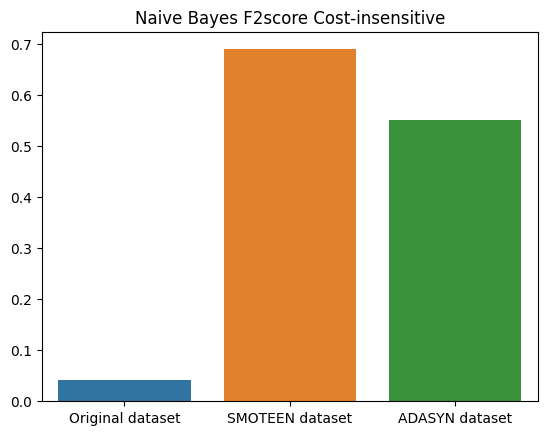
\includegraphics[scale=0.73]{Bayes}
		\end{figure}
	\end{center}
	
	In questo caso applicando con il Naive Bayes possiamo riscontrare un'enorme differenza tra le metriche del modello addestrato sul dataset originale e quelle dei modelli addestrati sui dataset ribilanciati, da notare che il modello addestrato sul dataset al quale è applicato lo SMOTEENN è risultato migliore ma leggermente al di sotto dei risultati ottenuti con il modello basato sull'albero di classificazione. \\
	\linebreak
	\linebreak
	
	\subsubsection{Cost-sensitive learning}
	\begin{center}
		\quad
		\begin{table}[h]
			\footnotesize
			\begin{tabular}{|p{2cm}|c|}
				\hline
				\multicolumn{2}{|c|}{Dataset originale}\\ \hline
				Accuracy & 0.782 \\ \hline
				Presicion & 0.916 \\ \hline
				Recall & 0.782 \\ \hline
				F-measure macro & 0.404 \\ \hline
				ROC Area & 0.866 \\ \hline  
				\end{tabular}
				\hfill
				\begin{tabular}{|p{2cm}|c|}
				\hline
				\multicolumn{2}{|c|}{SMOTEENN}\\ \hline
				Accuracy & 0.859 \\ \hline
				Presicion & 0.891 \\ \hline
				Recall & 0.859 \\ \hline
				F-measure macro & 0.858 \\ \hline
				ROC Area & 0.911 \\ \hline  
				\end{tabular}
					\hfill
			\begin{tabular}{|p{2cm}|r|} \hline
				\multicolumn{2}{|c|}{ADASYN}\\ \hline
				Accuracy & 0.829 \\ \hline
				Presicion & 0.868 \\ \hline
				Recall & 0.829 \\ \hline
				F-measure macro & 0.824 \\ \hline
				ROC Area & 0.877 \\ \hline  
			\end{tabular}
		\end{table}
		\begin{figure}[h]
			\centering
			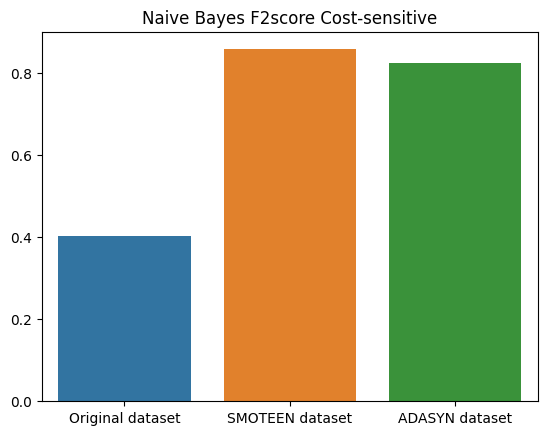
\includegraphics[scale=0.73]{BayesCostSens}
		\end{figure}
	\end{center}
	
	In questo caso, applicando il cost sensitive learning al Naive Bayes, possiamo notare un miglioramento nelle prestazioni del modello addestrato sul dataset originale, mentre i risultati per gli altri modelli sono leggermente superiori ai precedenti.
	
	\subsubsection{Considerazioni}
	Anche in questo, come il modello precedente, il miglioramento si nota intervenendo sulla distribuzione delle classi, ma anche applicando il cost-sensitive learning.
	
	
	\section{Conclusioni}
	Il nostro obiettivo principale era sviluppare un modello in grado di predire correttamente se un copro celeste rilevato vicino alla Terra fosse innoquo o meno per la stessa. Attraverso un'attenta analisi dei dati, l'ingegnerizzazione delle feature e l'addestramento di diversi modelli, siamo riusciti a raggiungere risultati significativi. \\
	\linebreak
	In primo luogo, abbiamo eseguito un'analisi esplorativa dei dati per comprendere la distribuzione delle variabili, identificare eventuali valori mancanti o outlier e comprendere le relazioni tra le feature. Successivamente, abbiamo effettuato una pre-elaborazione dei dati, andando ad eleminare attributi inutili ed affrontando il problema delle classi sbilanciate, sperimentando sulle varie combinazioni inerenti all'undersampling, oversampling sui dati e cost-sensitive leanring per gli algoritmi.\\
	\linebreak
	Abbiamo testato in particolare due tra i più famosi algoritmi di machine learning, tra cui decision tree (C4.5) e Naive Bayes, al fine di identificare il modello che ottenesse le migliori prestazioni in relazione alle diverse istanze del dataset. Dopo un'accurata validazione incrociata e l'ottimizzazione dei parametri, abbiamo selezionato l'algoritmo C4.5 come modello finale, avendo molti indicatori superiori al 90\%.\\
	\linebreak
	È importante sottolineare che, nonostante i risultati promettenti, ci sono ancora aree di miglioramento. Ad esempio, potremmo esplorare ulteriormente altre tecniche di feature engineering o considerare l'utilizzo di modelli di deep learning per ottenere risultati ancora migliori. \\
	\linebreak
	In conclusione, questa sperimentazione ha dimostrato che con una corretta pre-elaborazione e l'addestramento di modelli appropriati, è possibile ottenere risultati significativi. Tuttavia, ci sono ancora sfide e possibilità di miglioramento, che possono essere affrontate attraverso ulteriori ricerche.
	
\end{document}